%%
% Template for Assignment Reports
% 
%

\documentclass{article}

\usepackage{fancyhdr} % Required for custom headers
\usepackage{lastpage} % Required to determine the last page for the footer
\usepackage{extramarks} % Required for headers and footers
\usepackage{graphicx,color}
\usepackage{anysize}
\usepackage{amsmath}
\usepackage{natbib}
\usepackage{caption}
\usepackage{hyperref}
\usepackage{listings}
\usepackage{float}
\usepackage{lipsum}  
\usepackage{xcolor}
\usepackage{subcaption}

% Margins
%\topmargin=-0.45in
%\evensidemargin=0in
%\oddsidemargin=0in
\textwidth=6.5in
%\textheight=9.0in
%\headsep=0.25in 

\linespread{1.0} % Line spacing

\definecolor{codegreen}{rgb}{0,0.6,0}
\definecolor{codegray}{rgb}{0.5,0.5,0.5}
\definecolor{codepurple}{rgb}{0.58,0,0.82}
\definecolor{backcolour}{rgb}{0.95,0.95,0.92}

\lstdefinestyle{mystyle}{
    backgroundcolor=\color{backcolour},   
    commentstyle=\color{codegreen},
    keywordstyle=\color{magenta},
    numberstyle=\tiny\color{codegray},
    stringstyle=\color{codepurple},
    basicstyle=\ttfamily\footnotesize,
    breakatwhitespace=false,         
    breaklines=true,                 
    captionpos=b,                    
    keepspaces=true,                 
    numbers=left,                    
    numbersep=5pt,                  
    showspaces=false,                
    showstringspaces=false,
    showtabs=false,                  
    tabsize=2
}

\lstset{style=mystyle}

%%------------------------------------------------
%% Image and Listing code
%%------------------------------------------------
%%sw \includecode{caption for table of listings}{caption for reader}{filename}
\newcommand{\includecode}[3]{\lstinputlisting[float,floatplacement=H, caption={[#1]#2}, captionpos=b, frame=single]{#3}}


%%sw \includescalefigure{label}{short caption}{long caption}{scale}{filename}
\newcommand{\includescalefigure}[5]{
\begin{figure}[htb]
\centering
\includegraphics[width=#4\linewidth]{#5}
\captionsetup{width=.8\linewidth} 
\caption[#2]{#3}
\label{#1}
\end{figure}
}

%%sw \includefigure{label}{short caption}{long caption}{filename}
\newcommand{\includefigure}[4]{
\begin{figure}[htb]
\centering
\includegraphics{#4}
\captionsetup{width=.8\linewidth} 
\caption[#2]{#3}
\label{#1}
\end{figure}
}




%%------------------------------------------------
%% Parameters
%%------------------------------------------------
% Set up the header and footer
\pagestyle{fancy}
\lhead{\authorName} % Top left header
\chead{\moduleCode\ - \assignmentTitle} % Top center header
\rhead{\firstxmark} % Top right header
\lfoot{\lastxmark} % Bottom left footer
\cfoot{} % Bottom center footer
\rfoot{Page\ \thepage\ of\ \pageref{LastPage}} % Bottom right footer
\renewcommand\headrulewidth{0.4pt} % Size of the header rule
\renewcommand\footrulewidth{0.4pt} % Size of the footer rule
\setlength\parindent{0pt} % Removes all indentation from paragraphs

\newcommand{\assignmentTitle}{Lab 2} % Assignment title
\newcommand{\moduleCode}{CSU44061} 
\newcommand{\moduleName}{Machine Learning} 
\newcommand{\authorName}{Adriana\ Hrabowych} % Your name
\newcommand{\authorID}{19304296} % Your student ID
\newcommand{\reportDate}{\printDate}

%%------------------------------------------------
%%	Title Page
%%------------------------------------------------
\title{
\vspace{-1in}
\begin{figure}[!ht]
\flushleft

\includegraphics[width=0.4\linewidth]{reduced-trinity.png}
\end{figure}
\vspace{-0.5cm}
\hrulefill \\
\vspace{0.5cm}
\textmd{\textbf{\moduleCode\ \moduleName}}\\
\textmd{\textbf{\assignmentTitle}}\\
\vspace{0.5cm}
\hrulefill \\
}

\author{\textbf{\authorName,\ \authorID}}

\date{\today}



%%------------------------------------------------
%% Document
%%------------------------------------------------
\begin{document}
\lstset{language=Java, captionpos=b, frame=single, keywordstyle=\color{black}\bfseries, stringstyle=\ttfamily}
\captionsetup{width=.8\linewidth} 

\maketitle


%%------------------------------------------------
\section{Introduction}
In this assignment, the dataset used in part 'i' has the ID of 19-19-19-0 and the dataset used in part 'ii' has the ID of 19--38-19-0 .

\section{Part i }
\begin{center}
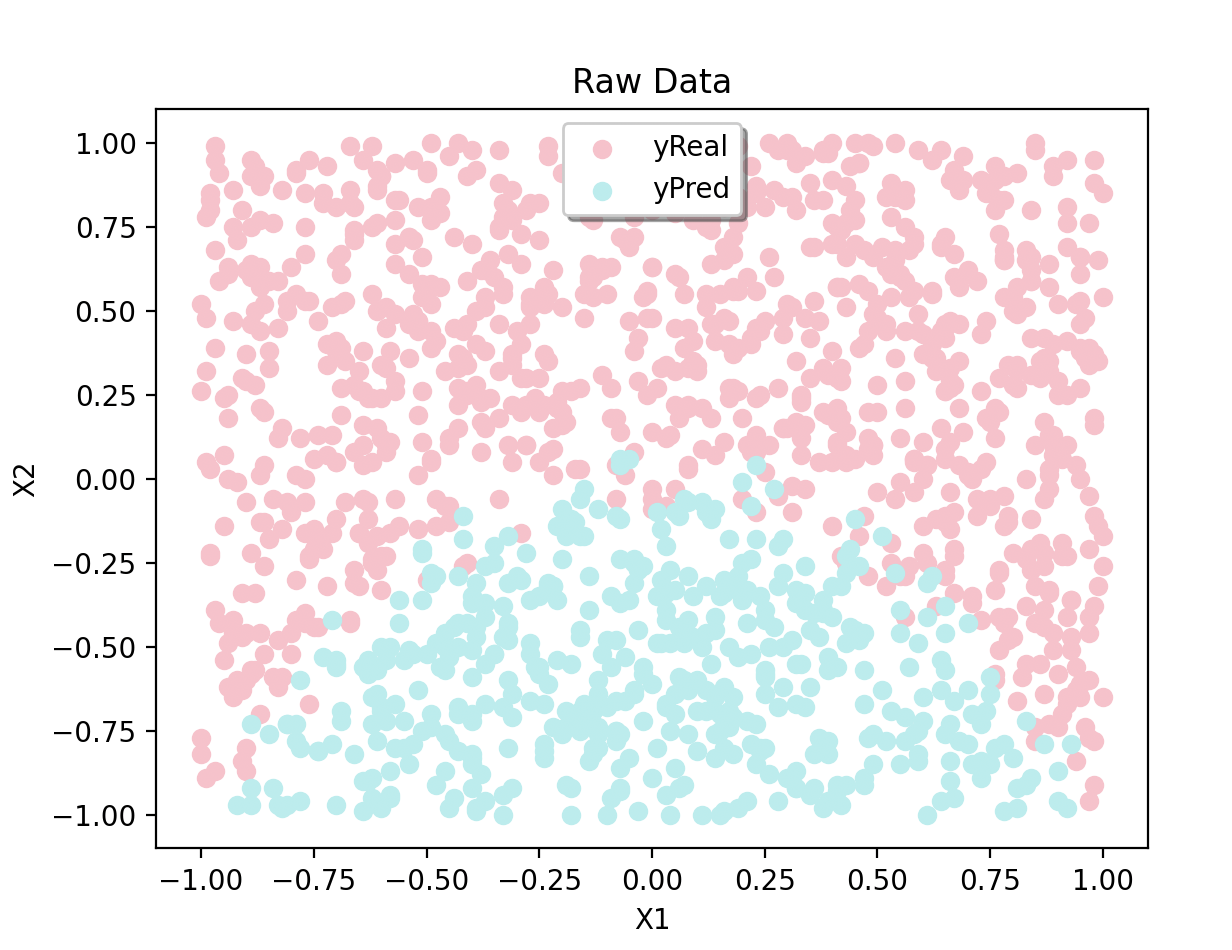
\includegraphics[width=.6\linewidth]{data1.png}
\end{center}
\captionof{figure}{A scatter plot graph visualizing the first dataset.}

\subsection{(i)(a)}
In (i)(a) we first read in the raw data and then visualize it on a graph as seen in figure one using circular markers. Each data point is placed depending on the value of its two features, with the X-axis corresponding to X1 and the Y-axis corresponding to X2. The color of the marker depends on the target value y, if the marker is red then y=1 and if blue then y=-1. As seen in figure one there is a clear decision boundary between the two classifications.

\begin{center}
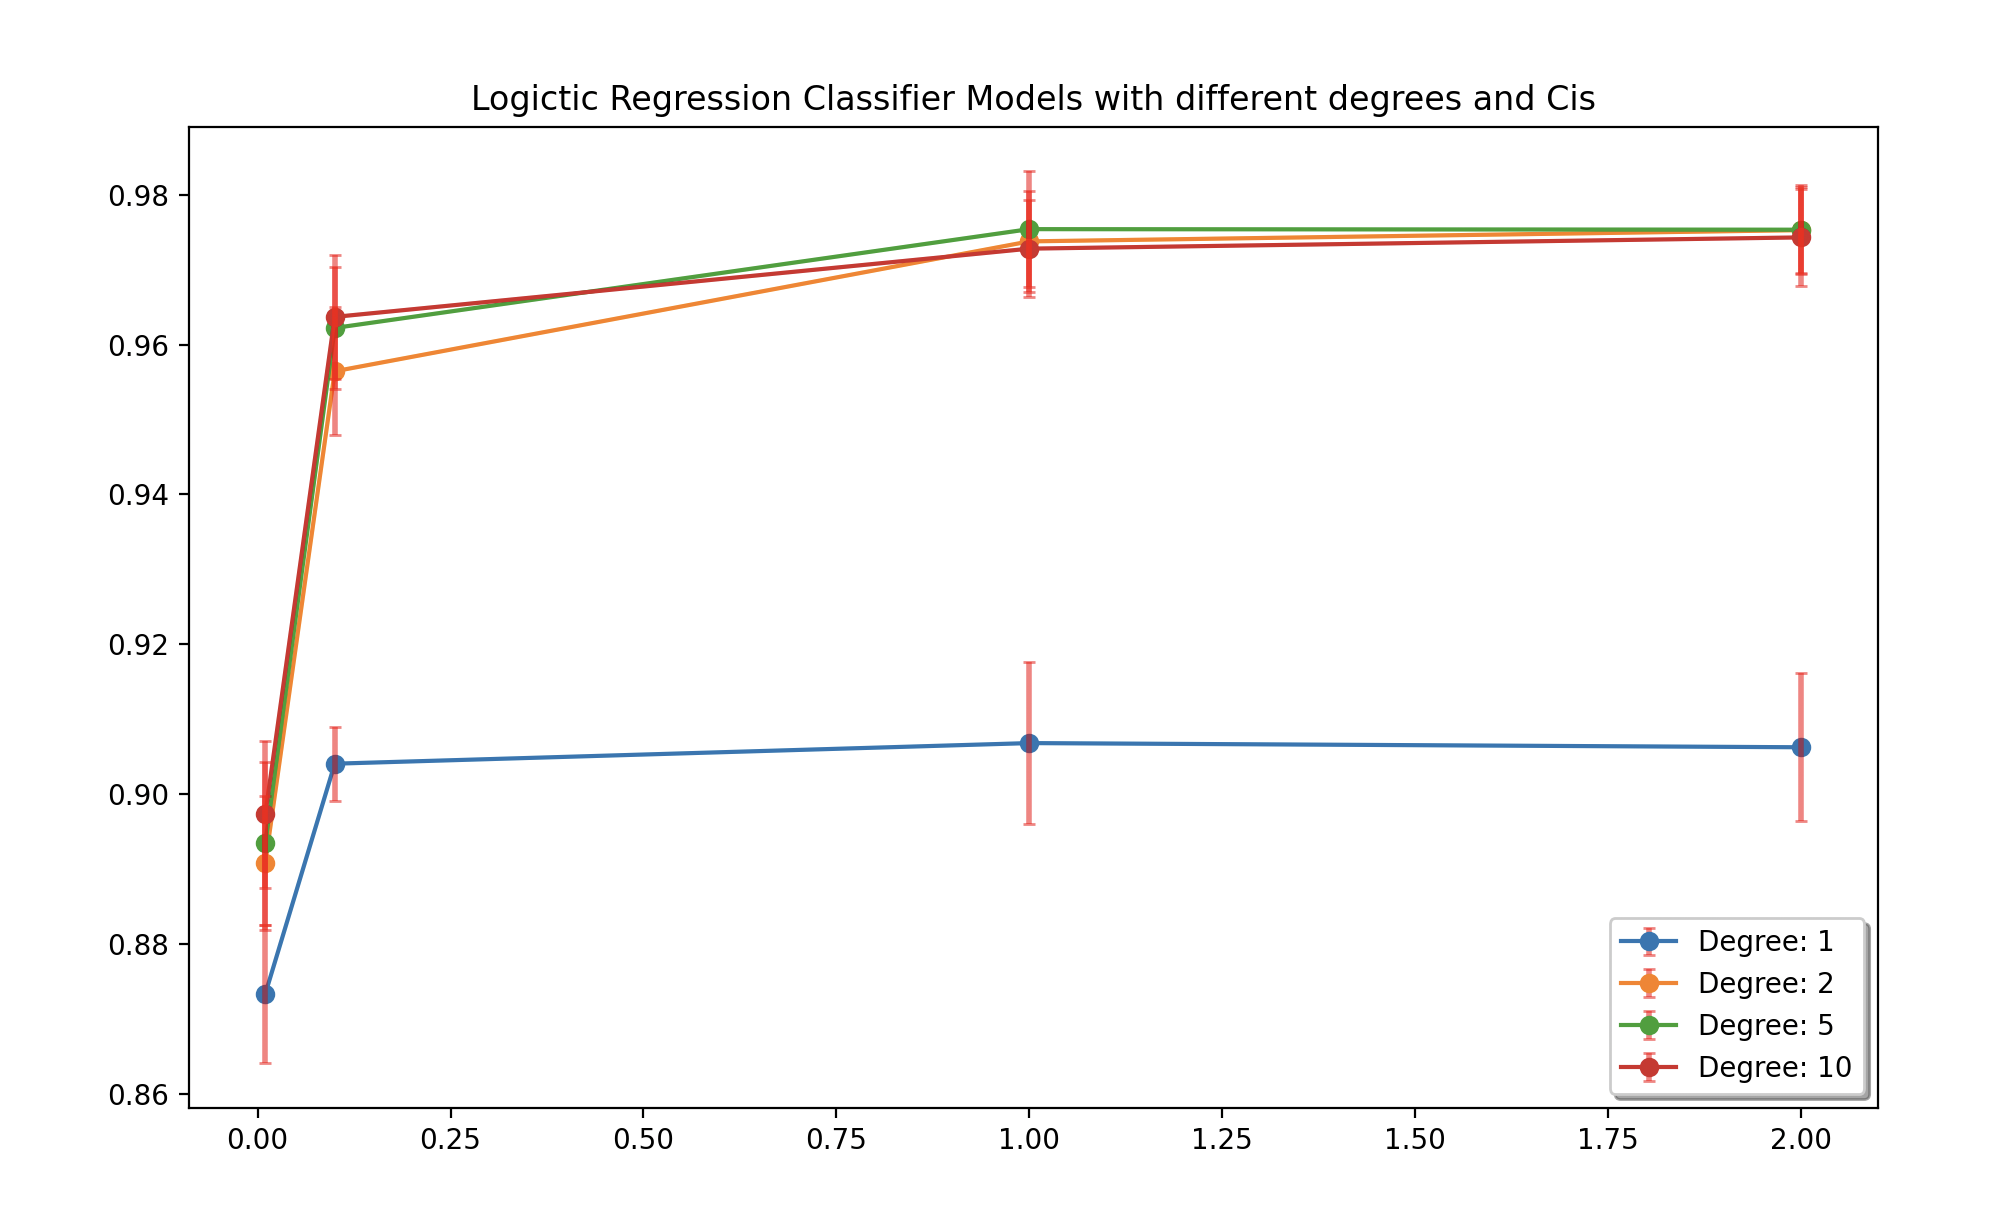
\includegraphics[width=\linewidth]{ia.png}
\end{center}
\captionof{figure}{A plot with four lines, each representing a Logistic model trained with a different polynomial degree of X. Each line has four points with an error bar, each of them represent the f1 score mean and standard deviation of a model with a different C value.}

In order to then train a logistic regression classifier on the data, we first have to use cross validation in order to choose the right polynomial degree of X and the correct weight for C. These are important to get right as the accuracy of a model can change drastically depending on the values.

During cross validation the range of polynomial degrees used was [1, 2, 5, 10]. I chose these values as they represent a good spread and represent the typical range of degrees used in logistic regression classifiers (which the addition of 1 and 10 as outliers). The range of C values used were [0.01, 0.1. 1, 2], chosen for the same reasons as the degrees. The default C used is typically 1, and then I added greater and lesser values to have a good spread.

The accuracy metric used in the following cross validation was the F1 score. The higher the score the better precision and recall a model has. The F1 score is calculated as:
\begin{center}
P = \# True Positives / (\# True Positives + \# False Positives)

R = \# True Positives / (\# True Positives + \# False Negative)

F1 Score = 2 * (P * R) / (P + R)
\end{center}
F1 scores were chosen as it combines both precision and recall and gives good results when the dataset is imbalanced (as ours is, see figure 1). Also, MSE cannot be used as a metric for classification as it cannot compare discrete classes.

The graph in figure two represents the outcomes of cross validation. A model was trained on each combination of C values and degrees, with a total of 16 models. A five-fold cross validation is performed on each model, the f1 score of each iteration is calculated and a mean and standard deviation f1 scores taken for each model. Five-fold cross validation was chosen as it is commonly used. 

As seen in figure two, the polynomial degree which consistently gives the higher f1 scores is five, and the C value which does the same is 1. Both of these outcomes make sense as these values are commonly the default for a logistic regression classifier.

\begin{center}
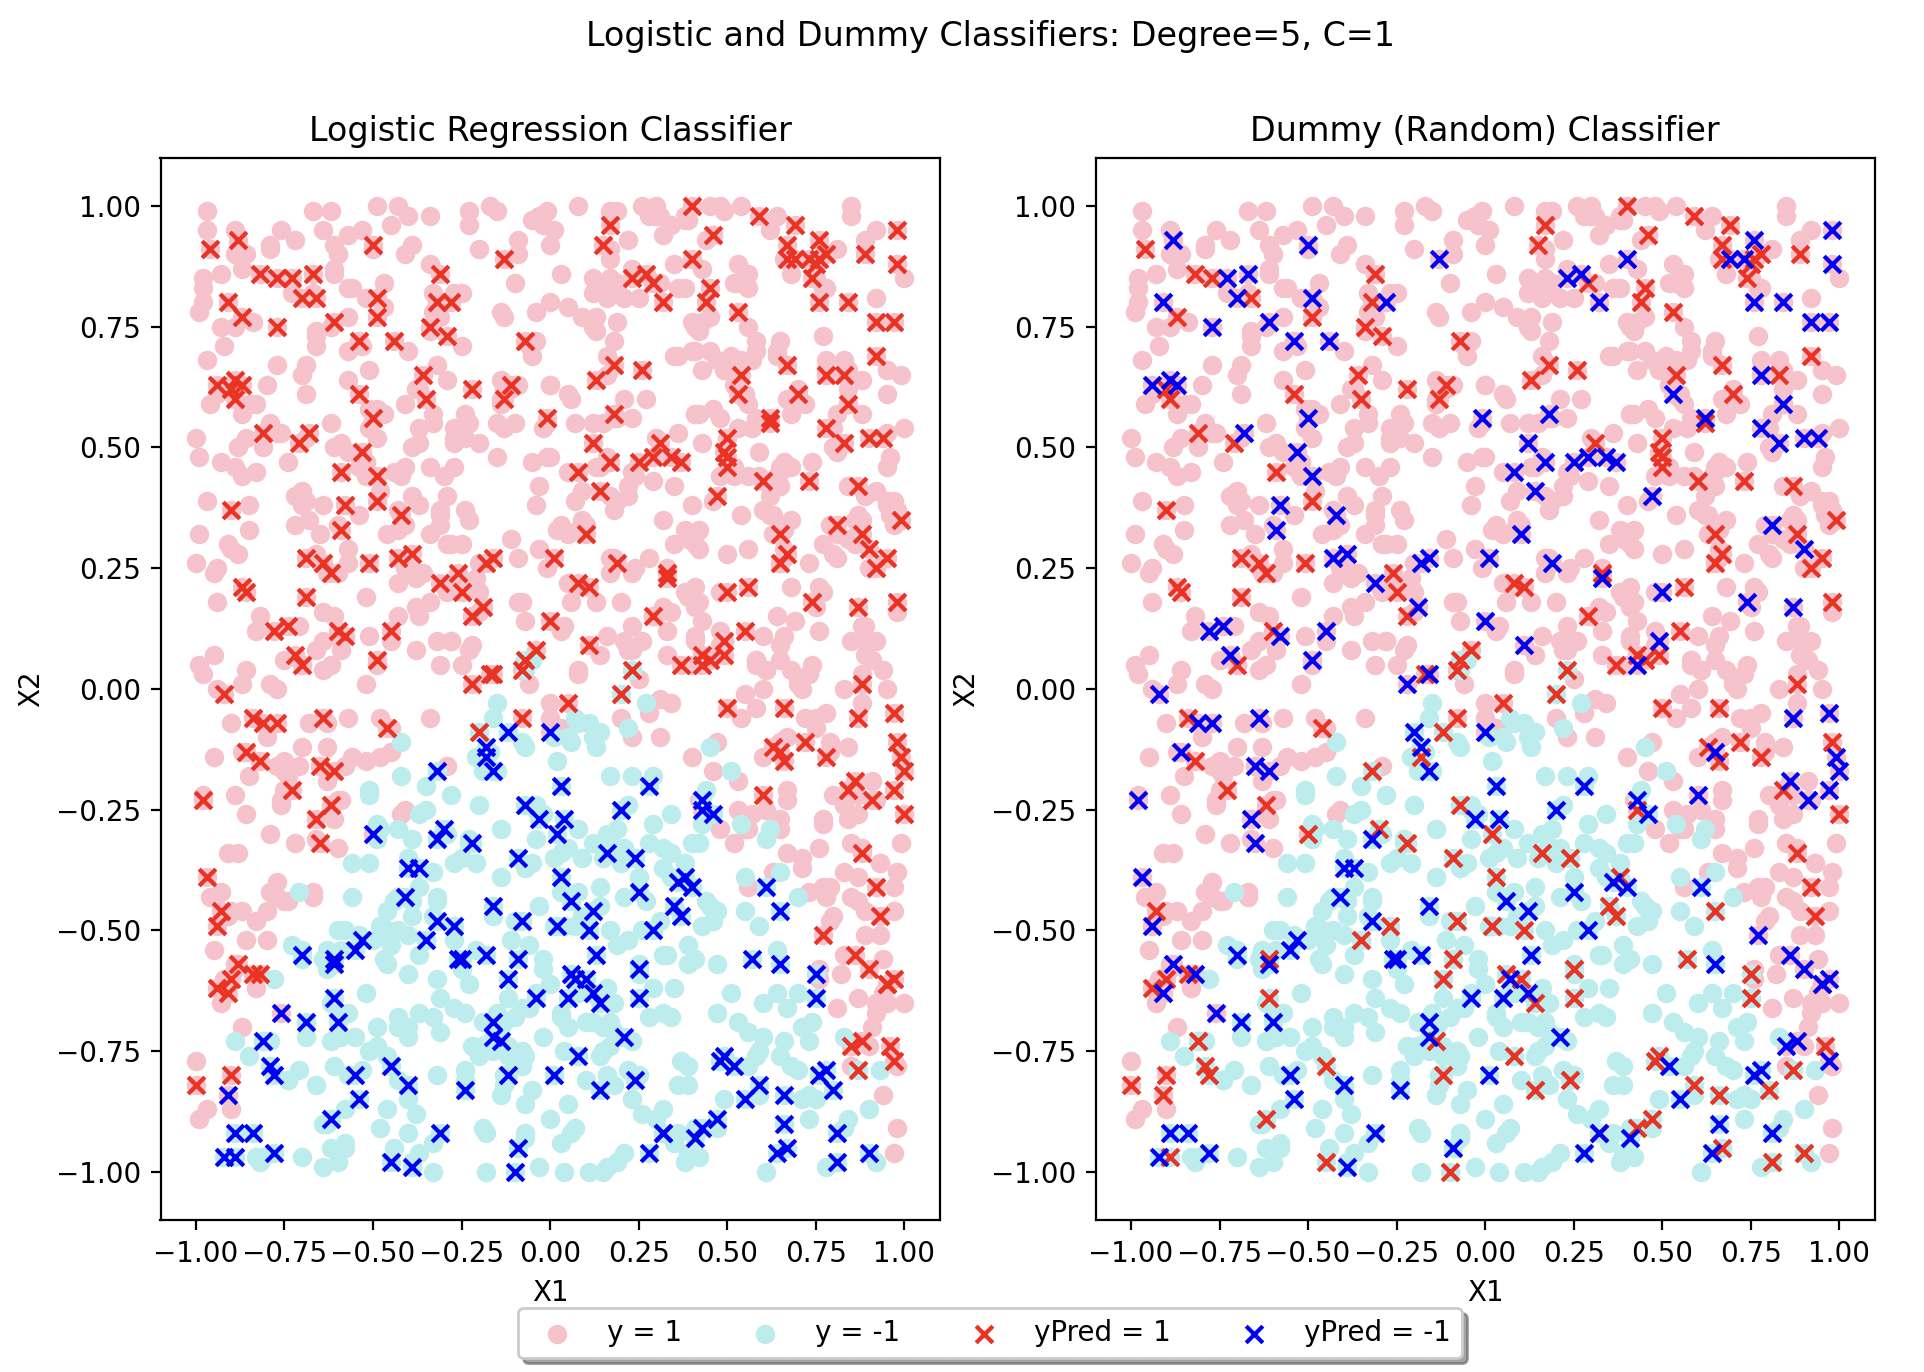
\includegraphics[width=\linewidth]{logreg.png}
\end{center}
\captionof{figure}{A figure with two scatter plots, the left one representing the predictions of the logistic regression classifier and the right being a random dummy model.}

The data is then split between training and testing and the features are brought to an order of five. A logistic regression model (with a C of 1) and a dummy model (using an uniform random classification) are then trained and told to predict the testing data. The outcome of this is seen in figure 3. The LRC performed much better than the dummy classifier, with the f1 scores of each being 0.97899 and 0.58095 respectively.

\subsection{(i)(b)}
We then train a K-nearest neighbors classifier on the data. Knn, a point is predicted based on the most frequent classification of the points around it. The parameter 'k' defines the number of neighbors to use, we will use cross validation to choose this value. It is important to choose the correct k as too small of a k leads to overfitting while a too big k leads to under-fitting. 

The values of k chosen for cross validation were [2, 5, 9, 14]. This spread was chosen as it represents both high, low, and 'typical' k's. Once again I used f1 scores and 5-fold cross validation. As there was only one value to cross validate instead of 2, there are only 4 models total. The outcome is shown in figure 4, from this graph we can see that a k of 5 and 9 produced the highest f1 scores, but 5 had a much lower standard deviation. As such we will be using a k of five in our optimal model.

The data is then split between training and testing sections. A knn model (with a k of 5) and a dummy model (using an uniform random classification) are then trained and told to predict the testing data. The outcome of this is seen in figure 5. The knn classifier performed much better than the dummy classifier, with the f1 scores of each being 0.97991 and 0.607305 respectively.

\begin{center}
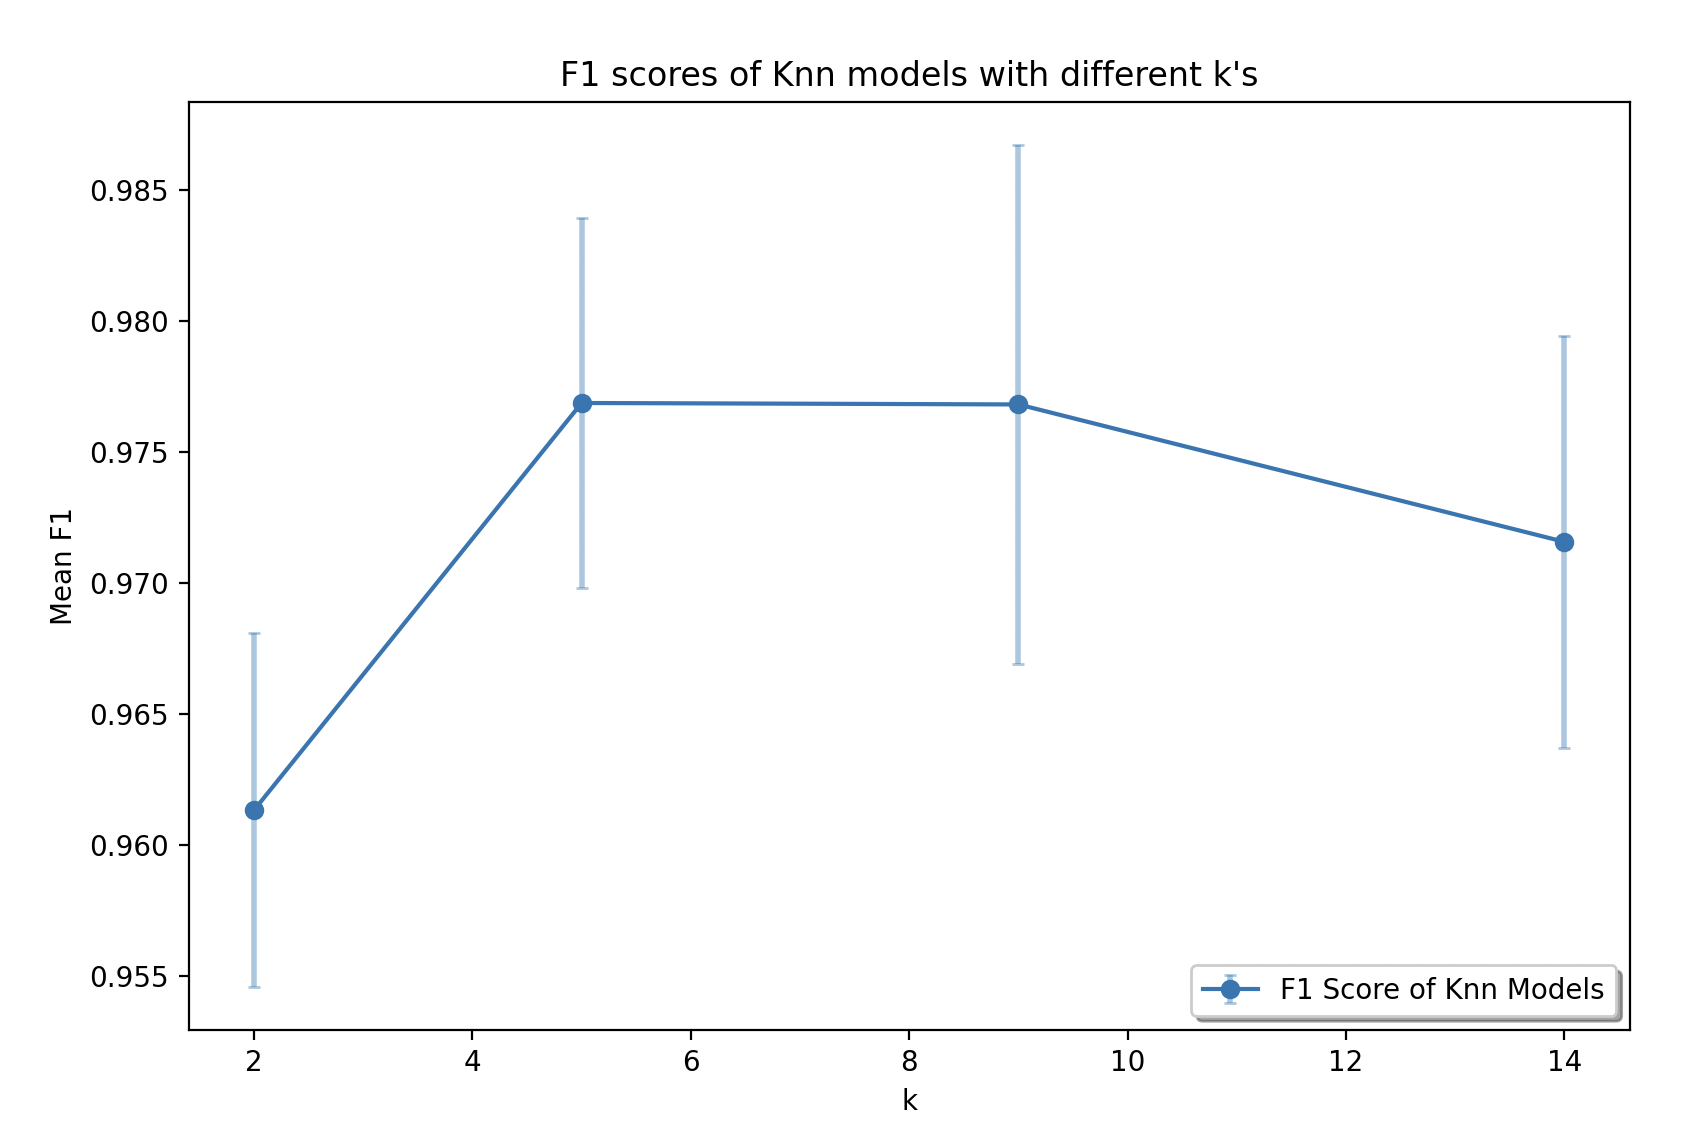
\includegraphics[width=.8\linewidth]{ib.png}
\end{center}
\captionof{figure}{A plot with a singular line with four points, each point has an error bar. It represents the mean f1 scores of a knn model with different values of k.}

\begin{center}
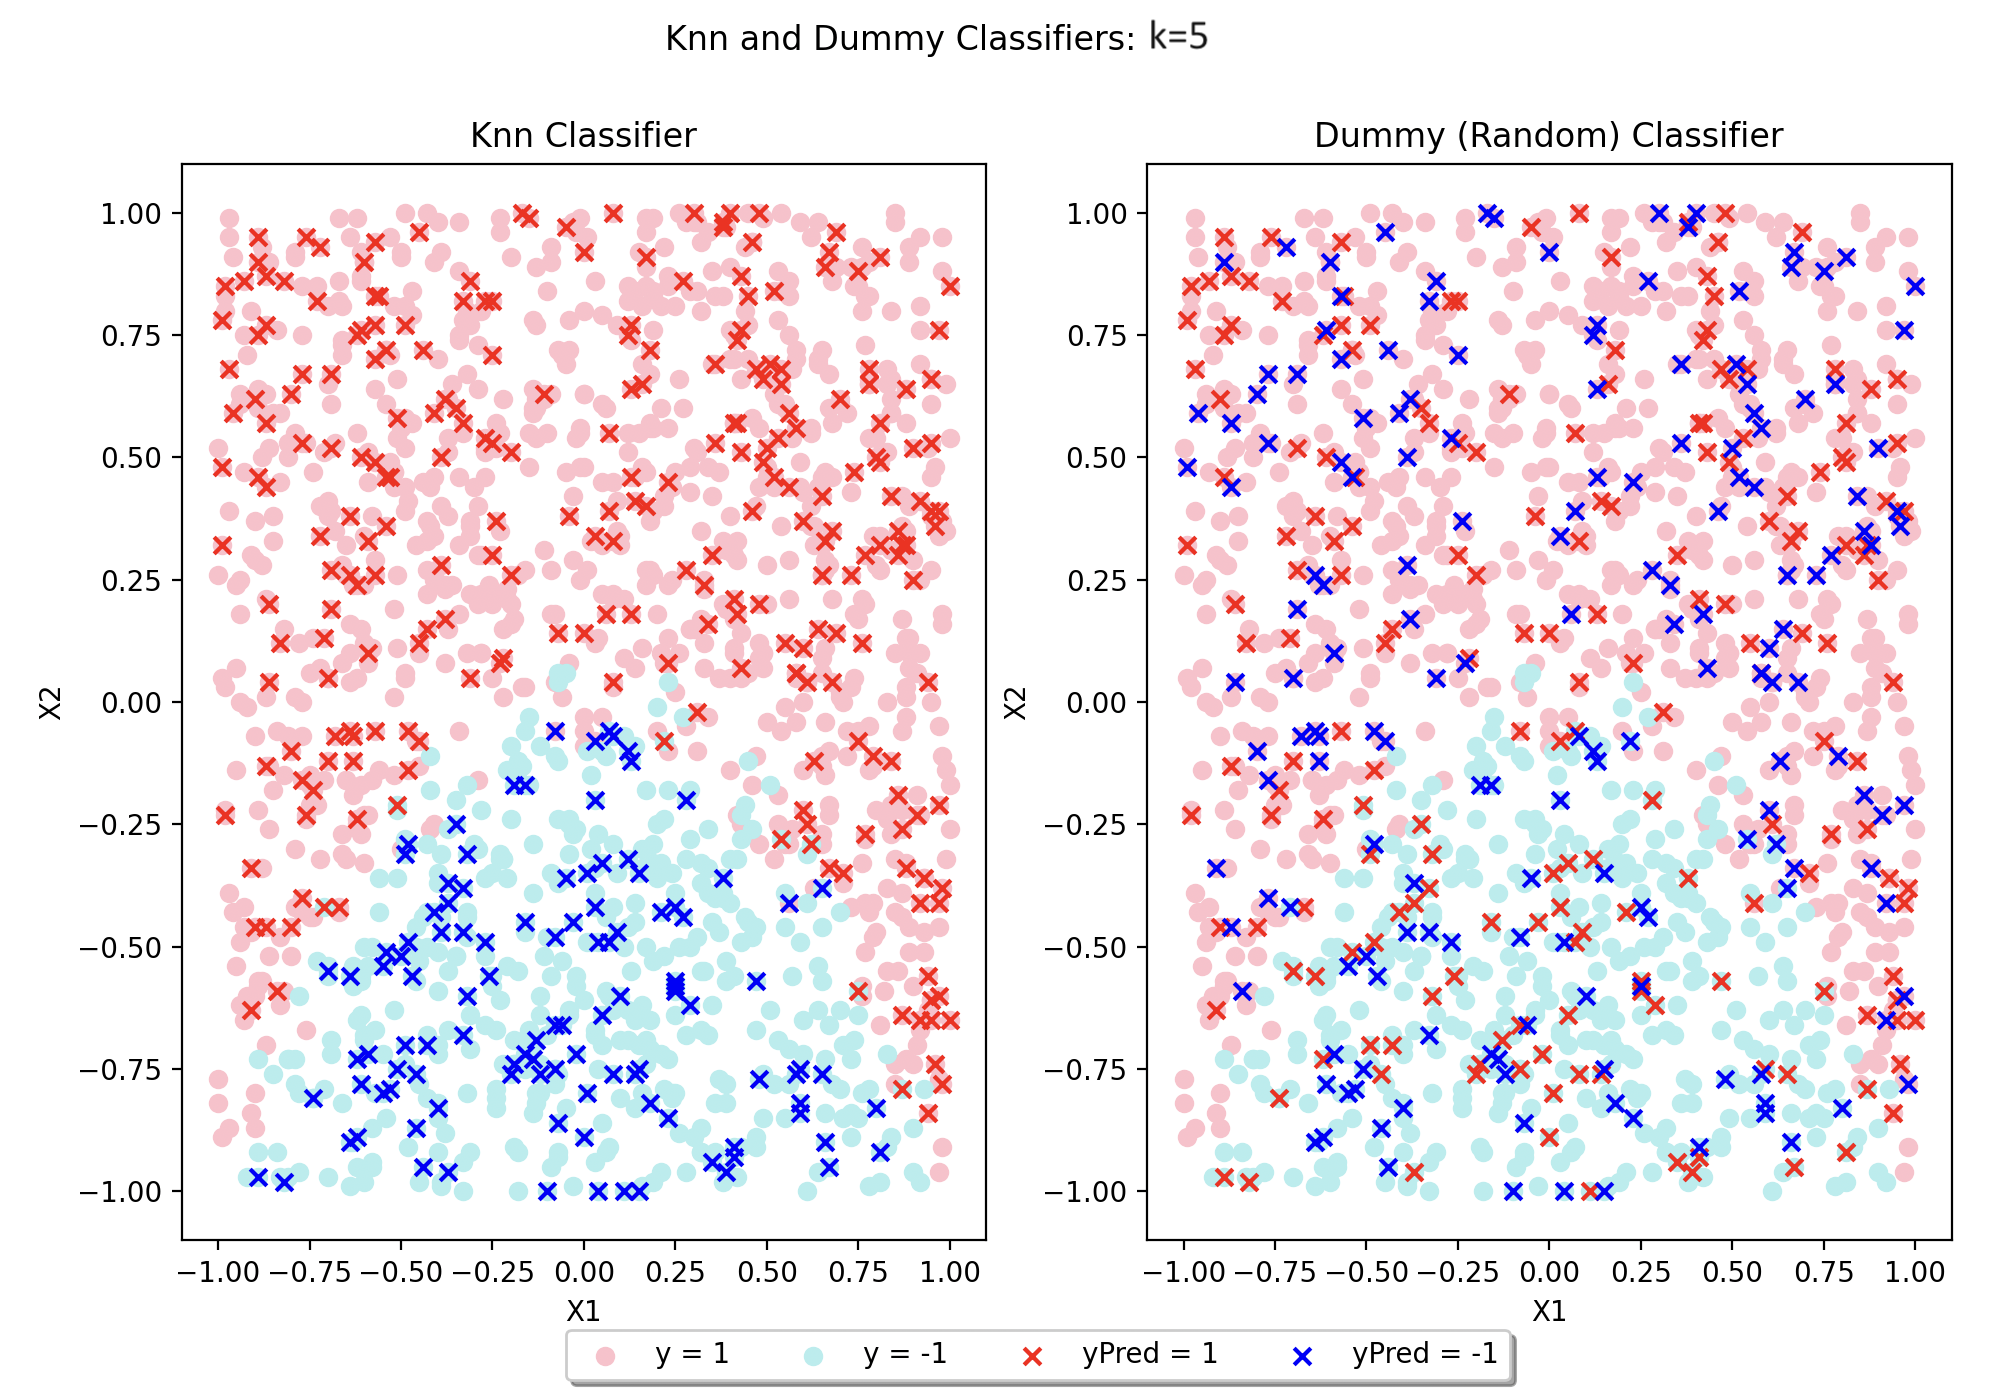
\includegraphics[width=\linewidth]{knn}
\end{center}
\captionof{figure}{A figure with two scatter plots, the left one representing the predictions of the knn classifier and the right being a random dummy model.}


\subsection{(i)(c)}
A confusion matrix is another type of performance metric that visualized the recall and precision in a table format. Data was split again between training and testing, and a LCR(C=1), Knn(k=5), and dummy (random) classifiers were all trained (with the LCR being trained with polynomial features to a degree of 5). They then made predictions based on the testing features and a confusion matrix was made by comparing those predictions to the real y values.

\begin{center}
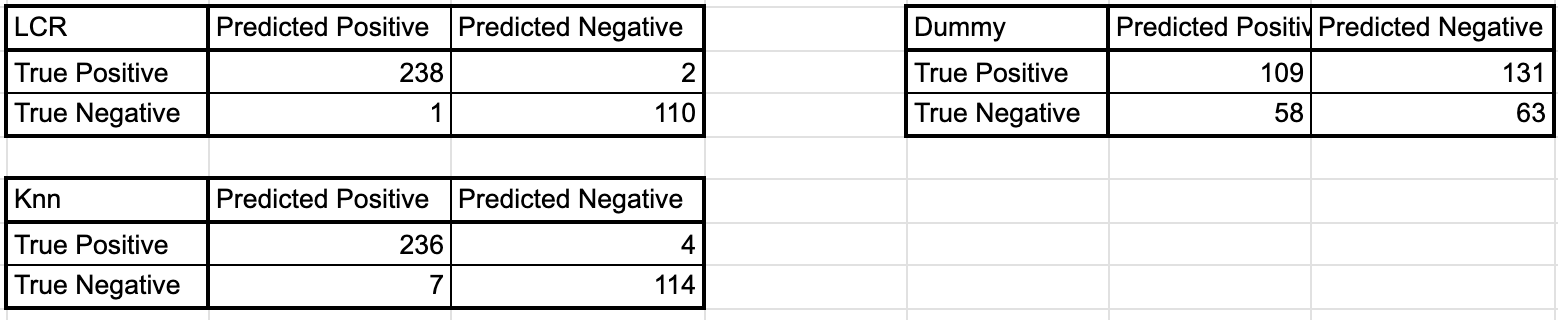
\includegraphics[width=\linewidth]{confusion.png}
\end{center}
\captionof{figure}{An image with 3 tables, each table being a confusion matrix for one of three models: LCR, Knn, and a dummy.}

\subsection{(i)(d)}
An ROC curve is line that plots the true positive rate of a model against the false positive rate of a model at different classification thresholds. A classification threshold is the threshold that must be reached for a model to classify a point as positive. The formula for each rate are as follows:
\begin{center}
TPR = TP / (TP + FN)

FPR = FP / (FP + TN)
\end{center}

Using the same data split and models as part C, the ROC curves of an LCR, Knn, and dummy model were plotted on the graph seen in figure 7.

\begin{center}
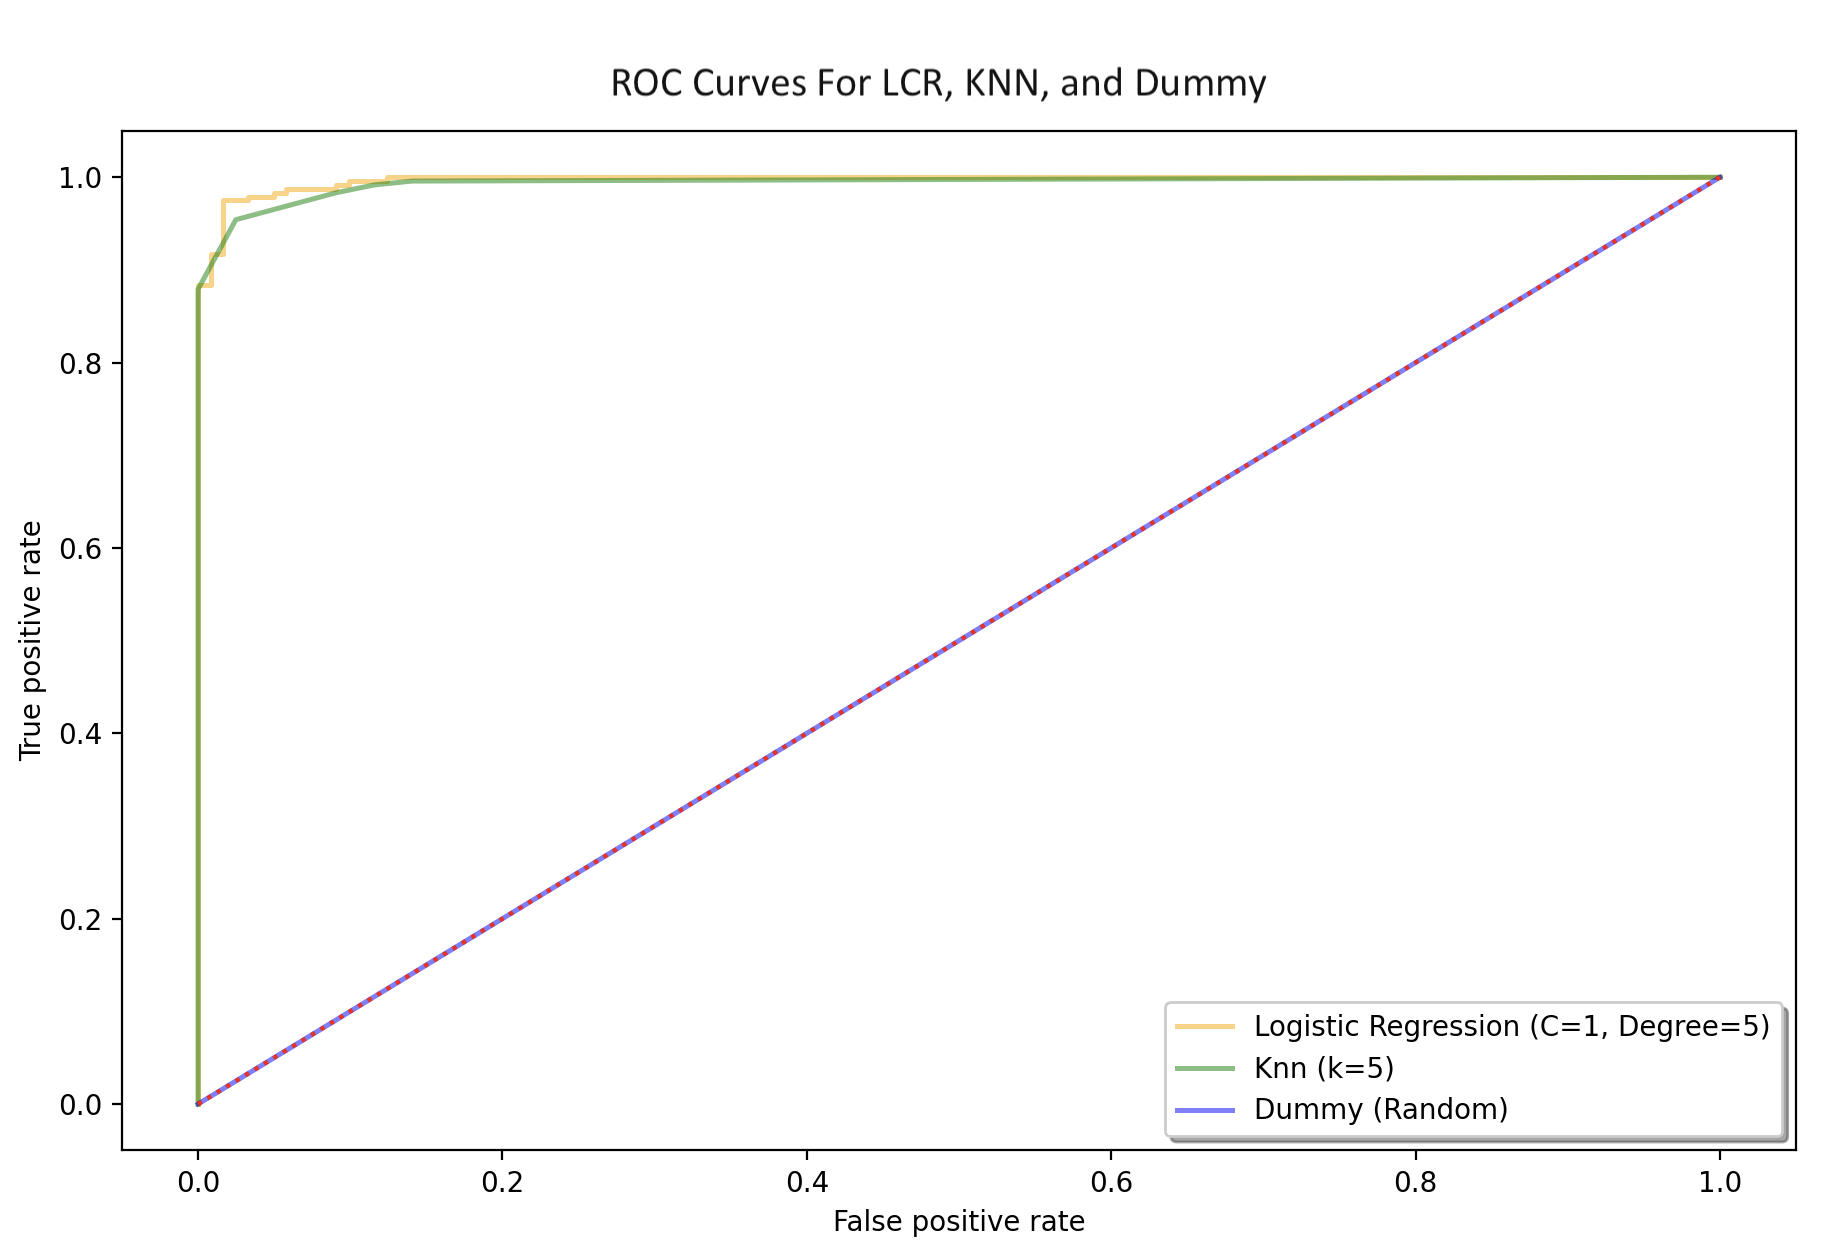
\includegraphics[width=.8\linewidth]{roc.png}
\end{center}
\captionof{figure}{A graph with four lines, each representing the roc curve of a LCR, knn, and dummy model with a baseline 1-1 also plotted.}

\subsection{(i)(e)}
The baseline dummy classifier performed far worse than both the LCR and Knn, as to be expected. It's confusion matrix had the most FPs and FNs and its ROC curve was practically the same as the baseline 1-1 line. The LCR performed slightly better than the Knn in the confusion matrix, as the number of FPs and FNS was only three, while Knn had 11 total. An ROC curve is considered better the closer the line is to an upside down L as it would mean that when the classification threshold is 1 the false positive rate is 0. The LCR again performs slightly better as it gets closer to the upper left corner than the Knn line does.
\\
\\
The f1 scores of each model are as follows: LCR = 0.97863, Knn = 0.97844, Dummy = 0.56937.
\\
\\
I would not be able to recommend a model for classification between the choice of LCR and Knn as the difference in the two in this example is not signifigant enough to be able to say for certain which is inherently better. 

\section{Part ii }
\subsection{(ii)(a)}
\begin{center}
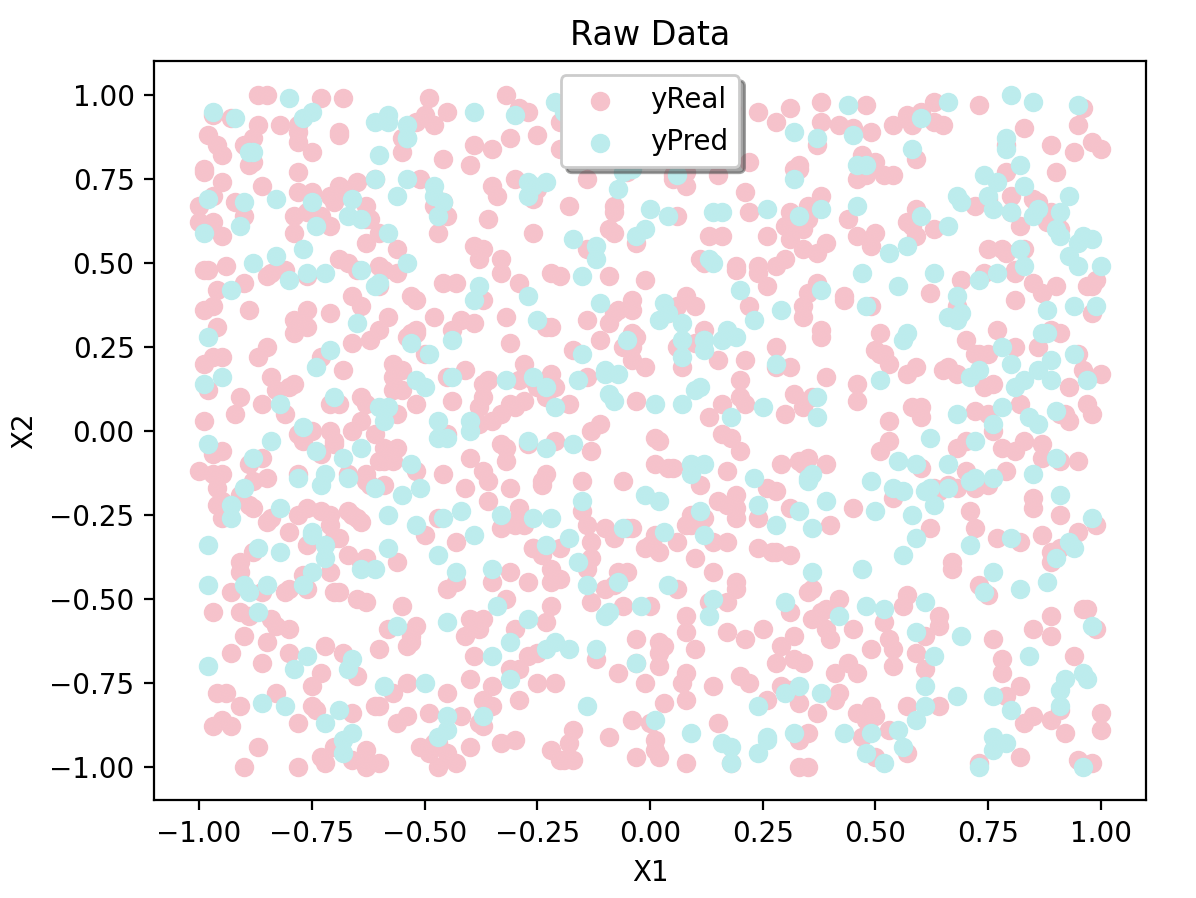
\includegraphics[width=.6\linewidth]{data2.png}
\end{center}
\captionof{figure}{A scatter plot graph visualizing the second dataset.}

In (ii)(a) we first read in the raw data and then visualize it on a graph as seen in figure one using circular markers. Each data point is placed depending on the value of its two features, with the X-axis corresponding to X1 and the Y-axis corresponding to X2. The color of the marker depends on the target value y, if the marker is red then y=1 and if blue then y=-1. As seen in figure 8, there is no clear decision boundary between the two classifications.

As in part (i)(a) we use the same form of cross validation with the same range of polynomial degrees and C values. The graph in figure 9 shows the outcomes of this cross validation. It is obvious from looking at the graph that this dataset does not seem to capture the same relationship as part i. Contrary to part (i) where the optimal degree was 5, for this dataset it seems to be 2. Though just barely as every combination of degree and C have extremely high standard deviations and have lower means than those in part (i)(a). The optimal C is either 0.1 or 1, we will use 1 as it is typically standard.

In figure 10 we can see the outcome of a LCR model with a C of 1 and degree 2 against a baseline random dummy model. It is interesting to note that the LCR model only ever predicted positive. The f1 scores were as follows: LCR = 0.81904, Dummy = 0.59893. The LCR still performed better than the dummy, but was much worse than in part i.

\begin{center}
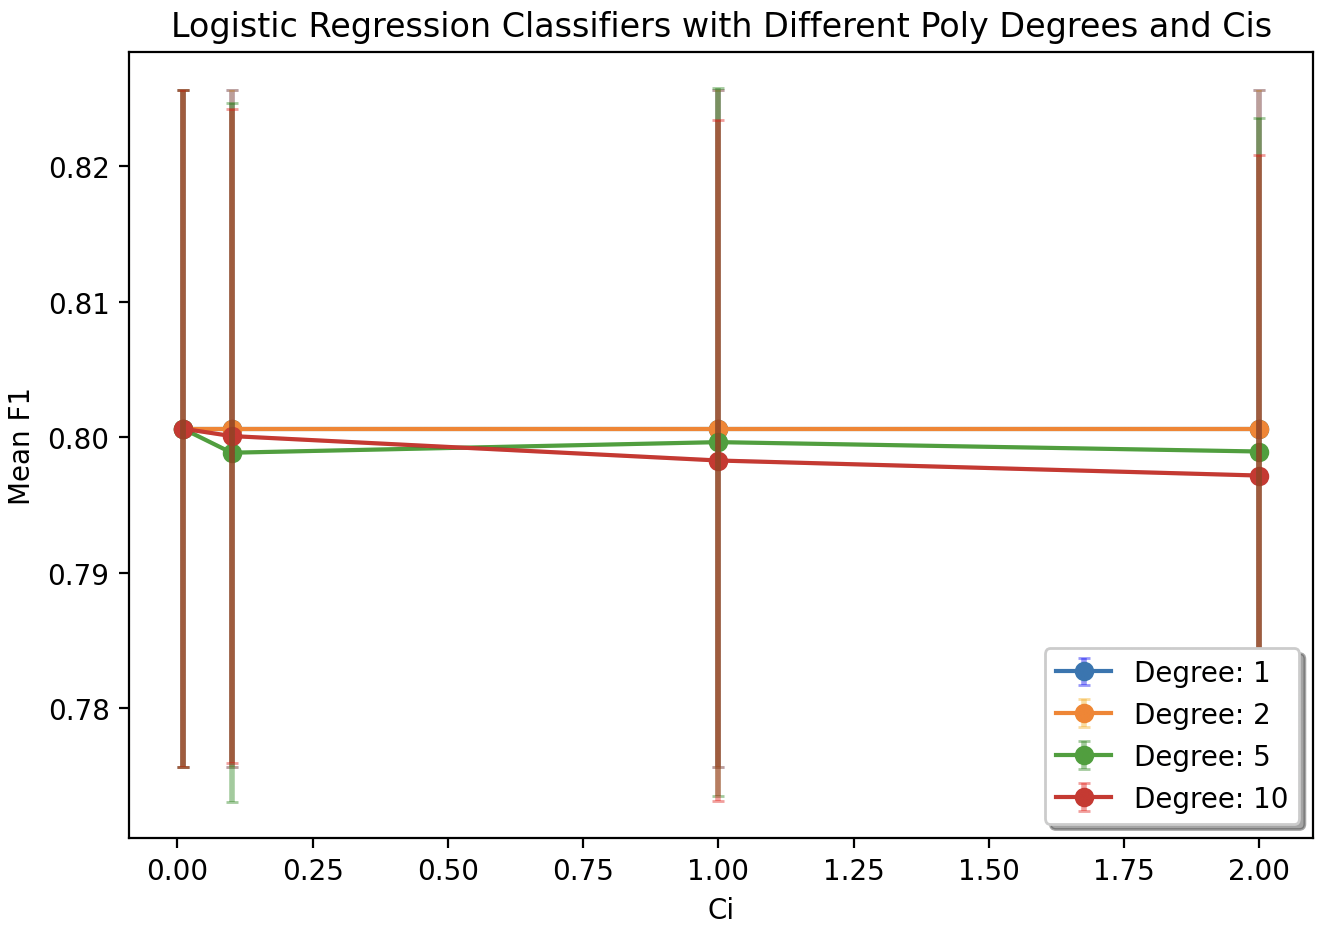
\includegraphics[width=.8\linewidth]{iia.png}
\end{center}
\captionof{figure}{A plot with four lines, each representing a Logistic model trained with a different polynomial degree of X. Each line has four points with an error bar, each of them represent the f1 score mean and standard deviation of a model with a different C value.}

\begin{center}
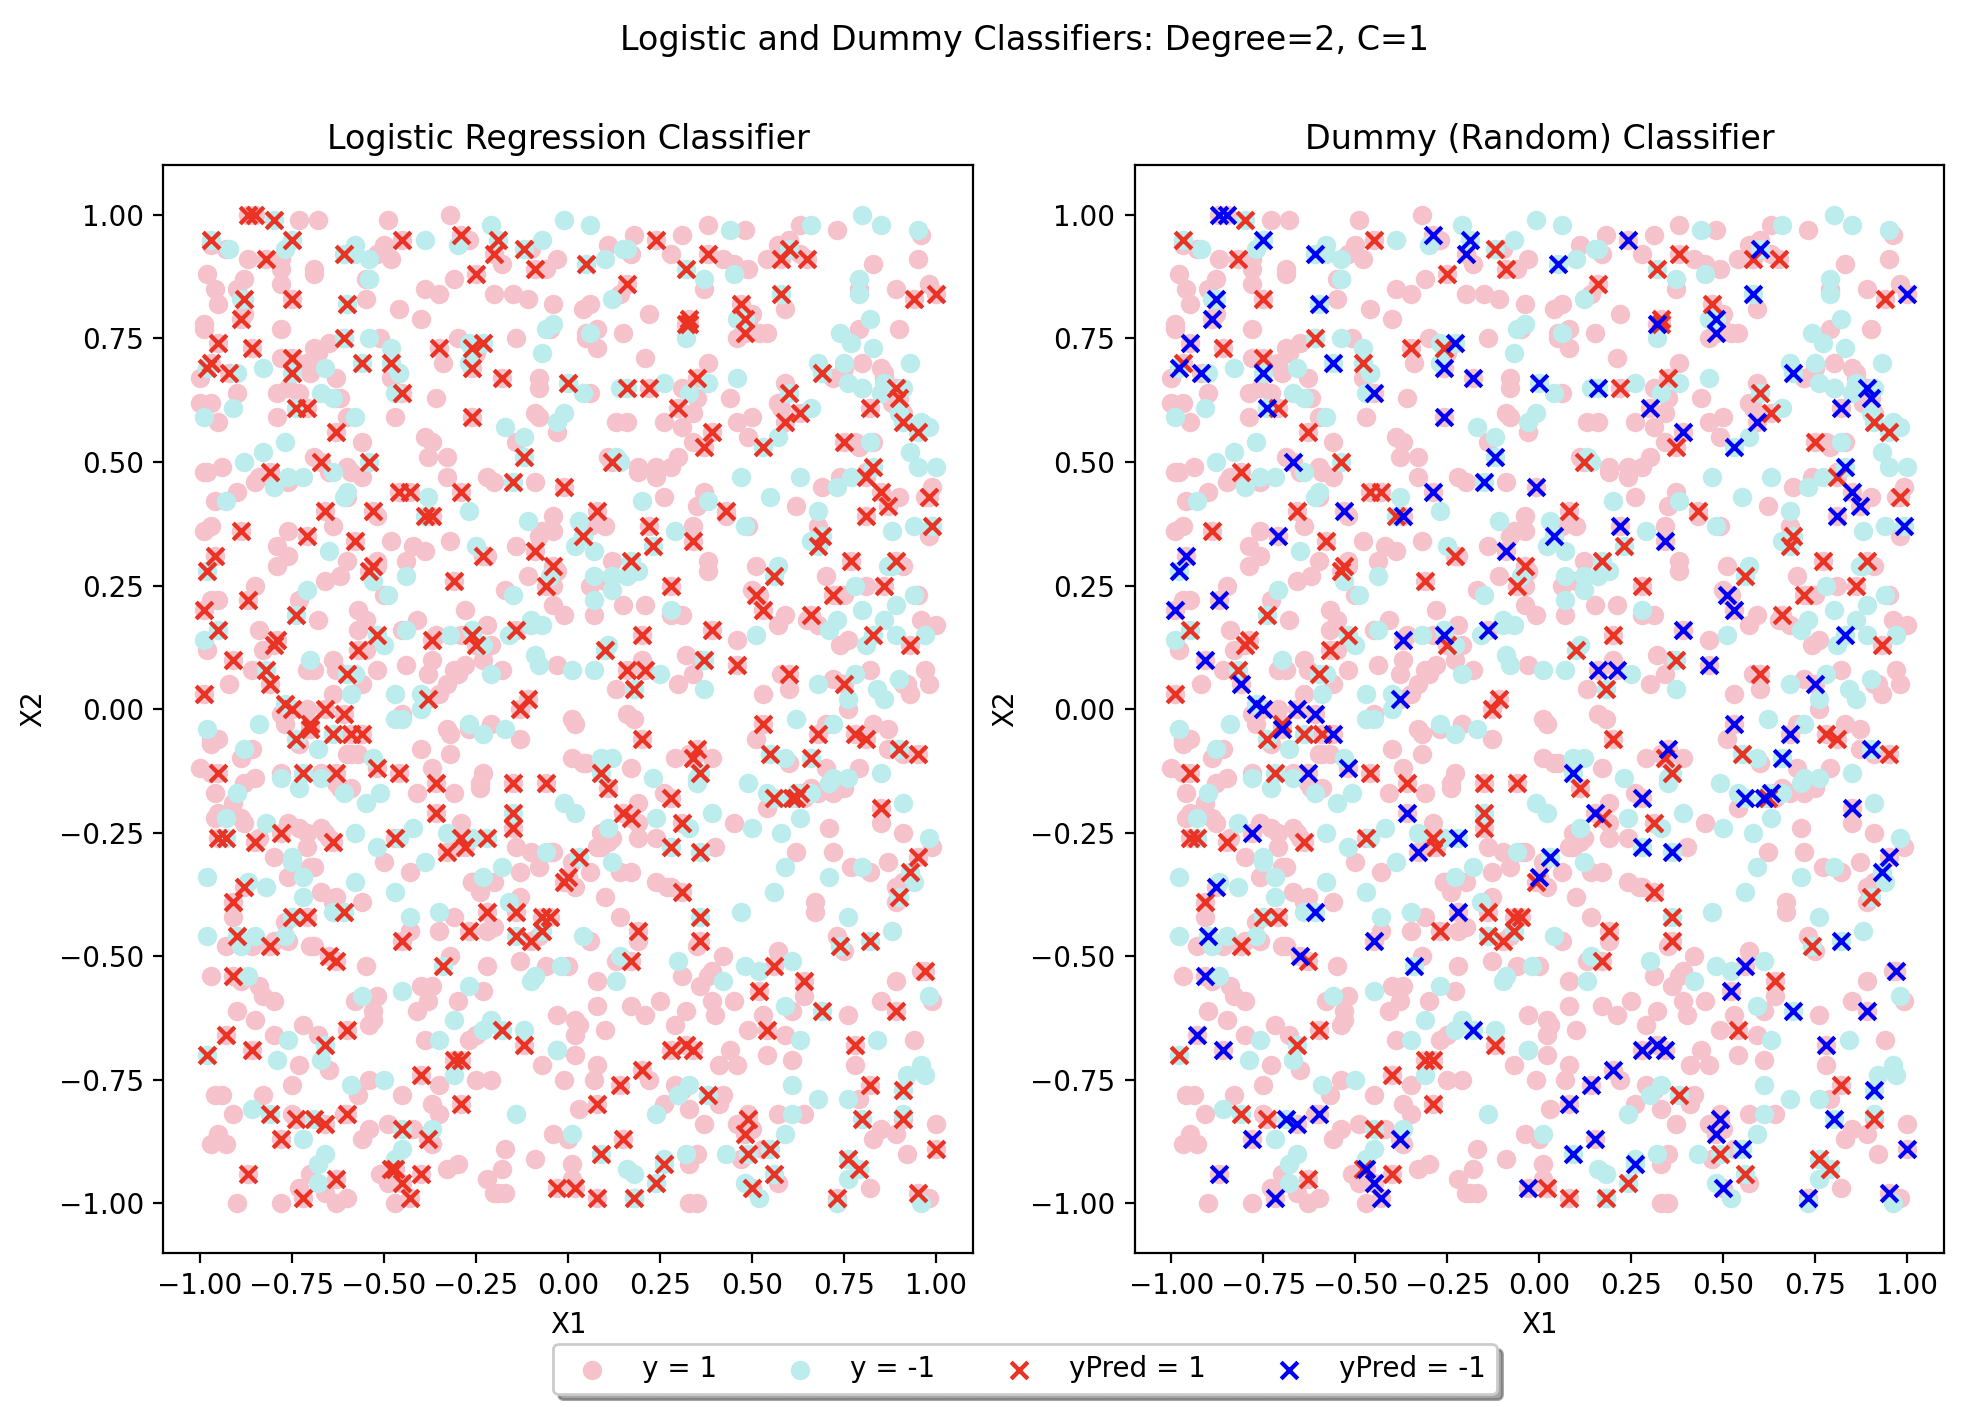
\includegraphics[width=.8\linewidth]{logreg2.png}
\end{center}
\captionof{figure}{A figure with two scatter plots, the left one representing the predictions of the logistic regression classifier and the right being a random dummy model.}

\subsection{(ii)(b)}
\begin{center}
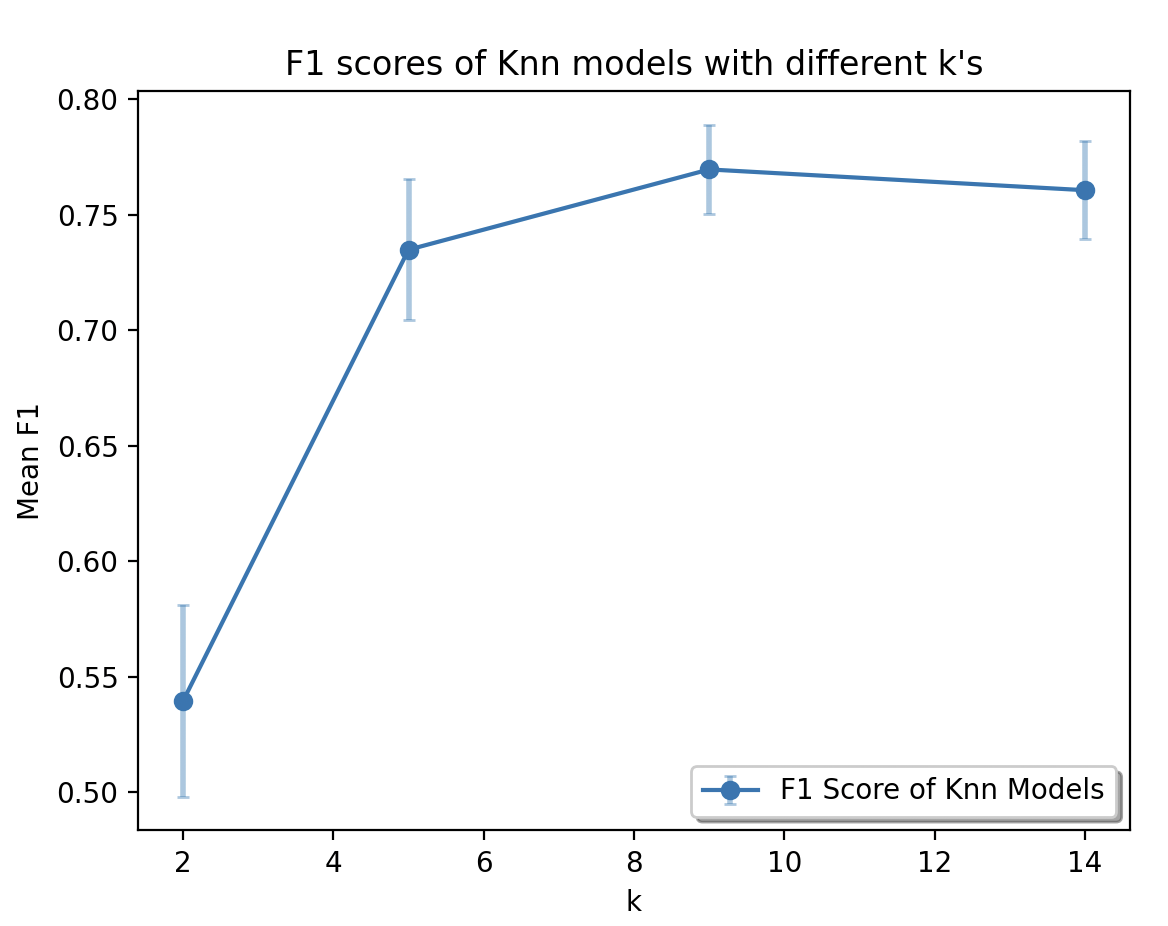
\includegraphics[width=.6\linewidth]{iib.png}
\end{center}
\captionof{figure}{A plot with a singular line with four points, each point has an error bar. It represents the mean f1 scores of a knn model with different values of k.}

\begin{center}
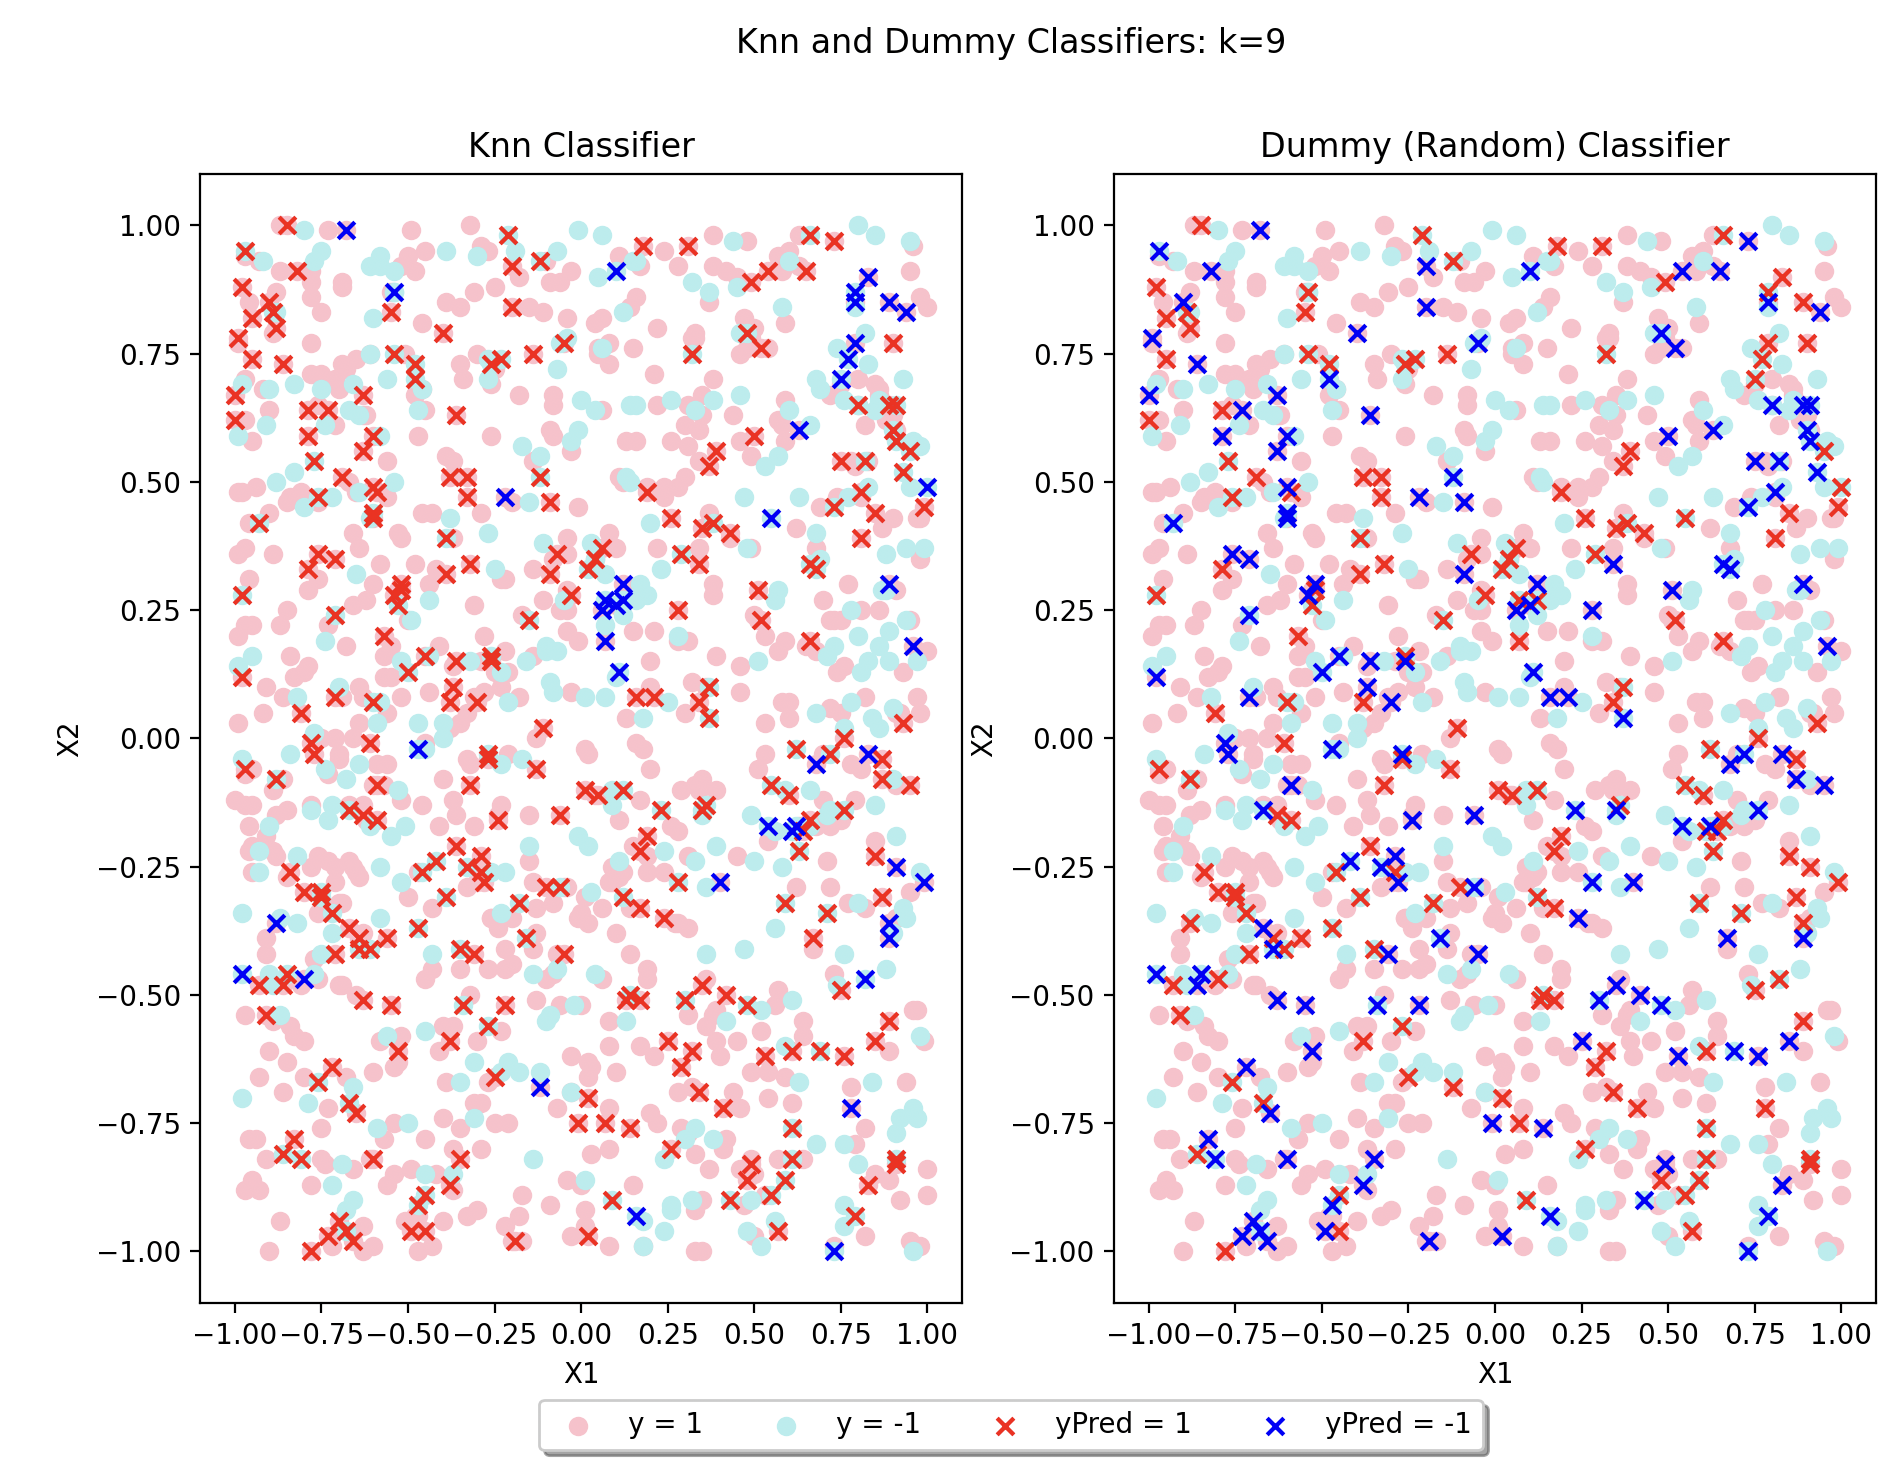
\includegraphics[width=.9\linewidth]{knn2}
\end{center}
\captionof{figure}{A figure with two scatter plots, the left one representing the predictions of the knn classifier and the right being a random dummy model.}

As in part (i)(b) we use the same form of cross validation with the same range of k values. The graph in figure 11 shows the outcome. The optimal K for this dataset seems to be 9, not 5 like in the previous part.

Once again we split the data and train a Knn model with a k of nine and a dummy model and then ask them to predict the test X's. The outcome of which is shown on figure 12. The f1 scores were as follows: Knn = 0.75213, Dummy = 0.5589. The Knn still performed better than the dummy, but was much worse than in part i.

\subsection{(ii)(c)}
Confusion matrices were made for the LCR (degree=2, C=1), Knn (k=9), and dummy models in the same way as in part i. They can be seen in figure 13.
\begin{center}
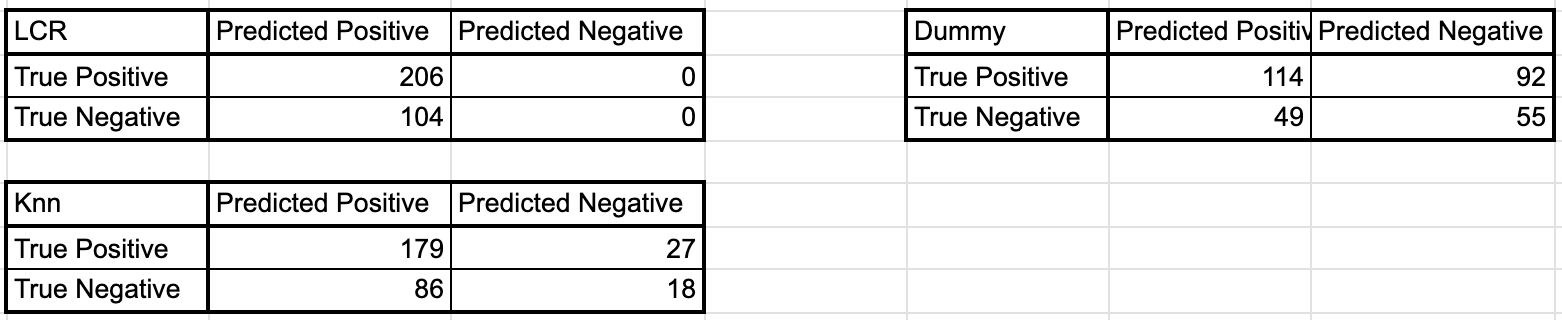
\includegraphics[width=\linewidth]{con}
\end{center}
\captionof{figure}{An image with 3 tables, each table being a confusion matrix for one of three models: LCR, Knn, and a dummy.}

\subsection{(ii)(d)}
Using the same data split and models as part C, the ROC curves of an LCR, Knn, and dummy model were plotted on the graph seen in figure 14.

\begin{center}
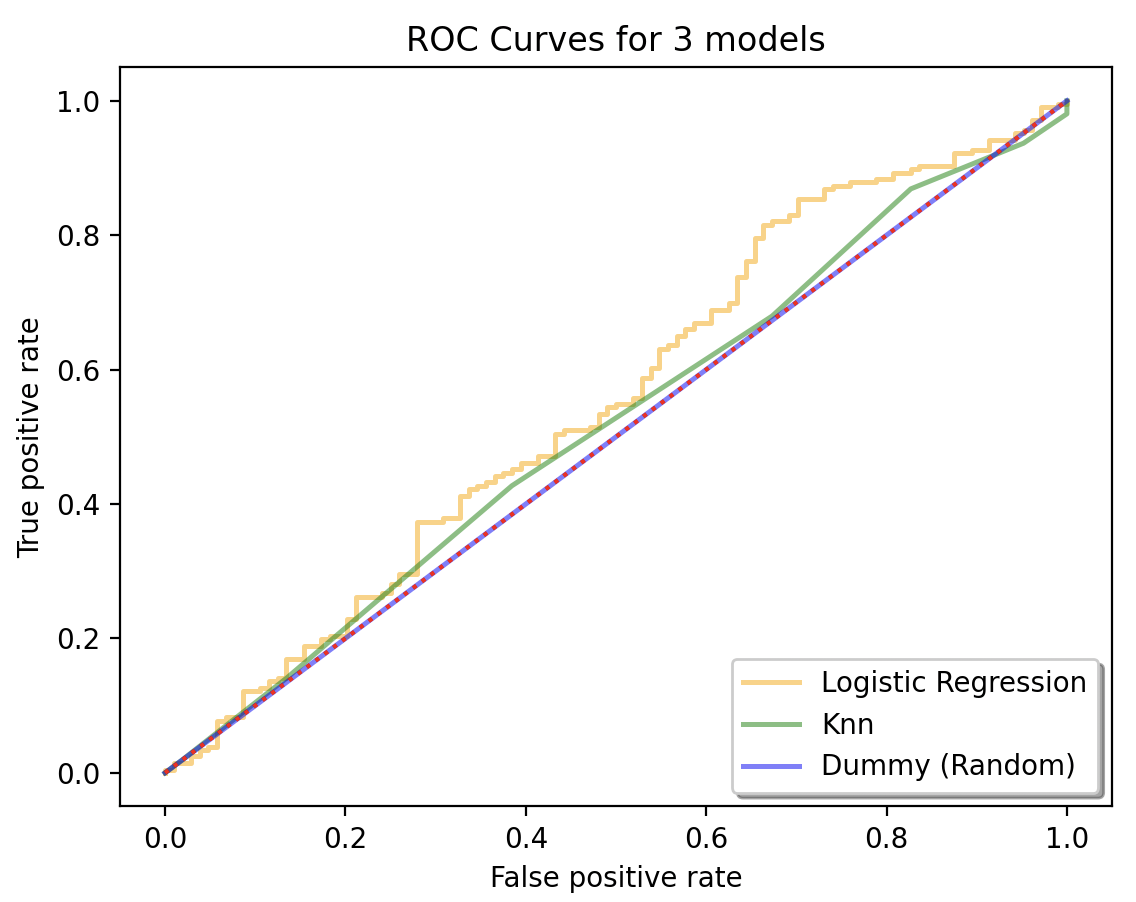
\includegraphics[width=.8\linewidth]{roc2.png}
\end{center}
\captionof{figure}{A graph with four lines, each representing the roc curve of a LCR, knn, and dummy model with a baseline 1-1 also plotted.}

\subsection{(ii)(e)}

The baseline dummy classifier performed worse than both the LCR and Knn, as to be expected. It's confusion matrix had the most FPs and FNs and its ROC curve was practically the same as the baseline 1-1 line. Both the LCR and Knn model performed far worse than in the previous parts, this is because the dataset is not useful and there wasn't any clear decision boundary between the two classifications. 
The LCR performed slightly better than the Knn in the confusion matrix, as the number of FPs and FNS was 104, while Knn had 113 total. Though it should be noted that the LCR strangely only predicted positive.The LCR again performs slightly better in the ROC graph as it gets closer to the upper left corner than the Knn line does.
\\
\\
The f1 scores of each model are as follows: LCR = 0.79844, Knn = 0.76008, Dummy = 0.572207.
\\
\\
I would not be able to recommend a model for classification between the choice of LCR and Knn as they both performed poorly and the difference in the two in this example is not significant enough to be able to say for certain which is better. This dataset is useless for classification and no classification model would be able to perform well.

\section{Appendix}
\lstinputlisting[language=Python]{../main.py}
\end{document}



